\documentclass[11pt]{article}
\usepackage{reotex}
\usepackage{verbatim}
\usepackage{pgf}
\usepackage{tikz}
\usepackage[pdftex]{hyperref}
\usepackage{url}


\title{A PGF-based Libary for Reo Circuits}
\author{\textbf{Nuno Oliveira}\\[12pt]HASLab/INESC TEC\\Universidade do Minho}
\date{\today}
\begin{document}
\maketitle


\begin{abstract}
This article briefly presents the package for Reo Circuits which is an \emph{extension} of the PGF/Tikz package, thoroughly documented in the manual ``Tikz \& PGF Manual for Version~2.10''.

Herein, the several commands to build a Reo circuit are presented and its \emph{API} explained.  

For a good usage of this package, \LaTeXe{} version is required. Some commands may work as well with \LaTeX{} version, but it is left as your responsibility.

Moreover, an excellent introduction to Reo can be found in~\cite{arbab04}, and for more information and tools on this theme the following website may be visited:
\begin{center}
\url{http://reo.project.cwi.nl/}
\end{center}

\end{abstract}


\section{How to Make it Work}

Ok, say you want to use this package to draw beautiful Reo Circuits. 
You start by loading your latex template. 
Then, in your preamble, you need to have the following:

\begin{itemize}
\item \verb+\usepackage{reotex}+
\end{itemize} 

Obviously, you need to have \verb+pgf+ and \verb+tikz+ packages installed in your environment, otherwise the commands provided in \verb+reotex+ will not be interpreted.


\section{Drawing a Reo Channel}

Reo circuits are the composition of several Reo channels. 
In this package all the channels have the same API, thus it is 
easy to explain a generic way of drawing such channels.

\subsection{The Generic Format}\label{sec:genericchannels}

The following pseudo-code shows how to draw any channel.

\begin{verbatim}
\tikz \<channel_name>{<start>} 
                    {<target>}
                    {<labels>} ;
\end{verbatim}

In detail, 
\begin{itemize}

\item \verb+\tikz+: refers to the Tikz environment to draw a tikz-based picture. In fact, the \verb+\tikz+ command is to draw an inline picture. If you desire to draw in a more controlled environment you may use:
\begin{verbatim}
  \begin{tikzpicture} 
      <channel name>{<start>}
                    {<target>}
                    {<labels>} 
  \end{tikzpicture}
\end{verbatim}

\item \emph{$<$channel name$>$}: refers to the command (representing the name of a channel) as presented in Section~\ref{sec:channels}.

\item \emph{$<$start$>$} refers to the coordinates of the starting point of the channel. It may be written either as $(x,y)$ or as a reference for a previous defined node: $(name)$. The second format should only be used in a tikzpicture environment.

\item \emph{$<$target$>$}: refers to the coordinates of the target point of the channel. It is used as the \emph{$<$start$>$} coordinate.

\item \emph{$<$labels$>$}: refer to the labels that may be desired to add to the channel. More than one label may be expressed; whenever it happens, a space should separate them. Each label should have the following format:

\begin{verbatim}
node[<options>] {<label>} ...
\end{verbatim}

where 

\begin{itemize}
\item \emph{$<$options$>$} are simple coma-separated graphic directives that may be used to transform the label. These directives are those used in normal \verb+pgf+ or \verb+tikz+ pictures: yshift=number, xshift=number, shift=number, color name, above, left, below and right, to list some but a few.

\item \emph{$<$label$>$} is the text to put on the channel. 
It may be used both simple text and mathematical text.

\end{itemize}

\end{itemize}


\subsection{Reo Channels}\label{sec:channels}

The following list presents the commands to draw the 22 defined Reo channels. 

\subsubsection{Synchronous Channels}

\indent

\begin{minipage}[b]{0.25\linewidth}
\verb+\sync+
\end{minipage}
\begin{minipage}[b]{0.2\linewidth}
\tikz \sync{(0,0)}{(1.5,0)}{}; 
\end{minipage}
\begin{minipage}[b]{0.6\linewidth}
\verb+\sync{(0,0)}{(1.5,0)}{}+ 
\end{minipage}

\medskip

\begin{minipage}[b]{0.25\linewidth}
\verb+\lossysync+
\end{minipage}
\begin{minipage}[b]{0.2\linewidth}
\tikz \lossysync{(0,0)}{(1.5,0)}{}; 
\end{minipage}
\begin{minipage}[b]{0.6\linewidth}
\verb+\lossysync{(0,0)}{(1.5,0)}{}+ 
\end{minipage}

\medskip

\begin{minipage}[b]{0.25\linewidth}
\verb+\syncdrain+
\end{minipage}
\begin{minipage}[b]{0.2\linewidth}
\tikz \syncdrain{(0,0)}{(1.5,0)}{}; 
\end{minipage}
\begin{minipage}[b]{0.6\linewidth}
\verb+\syncdrain{(0,0)}{(1.5,0)}{}+ 
\end{minipage}

\medskip

\begin{minipage}[b]{0.25\linewidth}
\verb+\syncspout+
\end{minipage}
\begin{minipage}[b]{0.2\linewidth}
\tikz \syncspout{(0,0)}{(1.5,0)}{}; 
\end{minipage}
\begin{minipage}[b]{0.6\linewidth}
\verb+\syncspout{(0,0)}{(1.5,0)}{}+ 
\end{minipage}

\medskip

\begin{minipage}[b]{0.25\linewidth}
\verb+\filter+
\end{minipage}
\begin{minipage}[b]{0.2\linewidth}
\tikz \filter{(0,0)}{(1.5,0)}{}; 
\end{minipage}
\begin{minipage}[b]{0.6\linewidth}
\verb+\filter{(0,0)}{(1.5,0)}{}+ 
\end{minipage}


\subsubsection{Asynchronous Channels}

\indent

\begin{minipage}[b]{0.25\linewidth}
\verb+\fifoe+
\end{minipage}
\begin{minipage}[b]{0.2\linewidth}
\tikz \fifoe{(0,0)}{(2,0)}{}; 
\end{minipage}
\begin{minipage}[b]{0.6\linewidth}
\verb+\fifoe{(0,0)}{(2,0)}{}+ 
\end{minipage}

\medskip

\begin{minipage}[b]{0.25\linewidth}
\verb+\fifof+
\end{minipage}
\begin{minipage}[b]{0.2\linewidth}
\tikz \fifof{(0,0)}{(2,0)}{}; 
\end{minipage}
\begin{minipage}[b]{0.6\linewidth}
\verb+\fifof{(0,0)}{(2,0)}{}+ 
\end{minipage}

\medskip

\begin{minipage}[b]{0.25\linewidth}
\verb+\asyncdrain+
\end{minipage}
\begin{minipage}[b]{0.2\linewidth}
\tikz \asyncdrain{(0,0)}{(2,0)}{}; 
\end{minipage}
\begin{minipage}[b]{0.6\linewidth}
\verb+\asyncdrain{(0,0)}{(2,0)}{}+ 
\end{minipage}

\medskip

\begin{minipage}[b]{0.25\linewidth}
\verb+\asyncspout+
\end{minipage}
\begin{minipage}[b]{0.2\linewidth}
\tikz \asyncspout{(0,0)}{(2,0)}{}; 
\end{minipage}
\begin{minipage}[b]{0.6\linewidth}
\verb+\asynspout{(0,0)}{(2,0)}{}+ 
\end{minipage}

\medskip

\begin{minipage}[b]{0.25\linewidth}
\verb+\fifon+
\end{minipage}
\begin{minipage}[b]{0.2\linewidth}
\tikz \fifon{(0,0)}{(2,0)}{}; 
\end{minipage}
\begin{minipage}[b]{0.6\linewidth}
\verb+\fifon{(0,0)}{(2,0)}{}+ 
\end{minipage}

\medskip

\begin{minipage}[b]{0.25\linewidth}
\verb+\shiftfifon+
\end{minipage}
\begin{minipage}[b]{0.2\linewidth}
\tikz \shiftfifon{(0,0)}{(2,0)}{}; 
\end{minipage}
\begin{minipage}[b]{0.6\linewidth}
\verb+\shiftfifon{(0,0)}{(2,0)}{}+ 
\end{minipage}

\medskip

\begin{minipage}[b]{0.25\linewidth}
\verb+\lossyfifon+
\end{minipage}
\begin{minipage}[b]{0.2\linewidth}
\tikz \lossyfifon{(0,0)}{(2,0)}{}; 
\end{minipage}
\begin{minipage}[b]{0.6\linewidth}
\verb+\lossyfifon{(0,0)}{(2,0)}{}+ 
\end{minipage}

\medskip

\begin{minipage}[b]{0.25\linewidth}
\verb+\timer+
\end{minipage}
\begin{minipage}[b]{0.2\linewidth}
\tikz \timer{(0,0)}{(2,0)}{}; 
\end{minipage}
\begin{minipage}[b]{0.6\linewidth}
\verb+\timer{(0,0)}{}{(2,0)}+ 
\end{minipage}

\medskip

\begin{minipage}[b]{0.25\linewidth}
\verb+\ordered+
\end{minipage}
\begin{minipage}[b]{0.2\linewidth}
\tikz \ordered{(0,0)}{(2,0)}{}; 
\end{minipage}
\begin{minipage}[b]{0.6\linewidth}
\verb+\ordered{(0,0)}{}{(2,0)}+ 
\end{minipage}

\medskip

\begin{minipage}[b]{0.25\linewidth}
\verb+\orderedn+
\end{minipage}
\begin{minipage}[b]{0.2\linewidth}
\tikz \orderedn{(0,0)}{(2,0)}{}; 
\end{minipage}
\begin{minipage}[b]{0.6\linewidth}
\verb+\orderedn{(0,0)}{(2,0)}{}+ 
\end{minipage}

\medskip

\begin{minipage}[b]{0.25\linewidth}
\verb+\bag+
\end{minipage}
\begin{minipage}[b]{0.2\linewidth}
\tikz \bag{(0,0)}{(2,0)}{}; 
\end{minipage}
\begin{minipage}[b]{0.6\linewidth}
\verb+\bag{(0,0)}{(2,0)}{}+ 
\end{minipage}

\medskip

\begin{minipage}[b]{0.25\linewidth}
\verb+\bagn+
\end{minipage}
\begin{minipage}[b]{0.2\linewidth}
\tikz \bagn{(0,0)}{(2,0)}{}; 
\end{minipage}
\begin{minipage}[b]{0.6\linewidth}
\verb+\bagn{(0,0)}{(2,0)}{}+ 
\end{minipage}

\medskip

\begin{minipage}[b]{0.25\linewidth}
\verb+\set+
\end{minipage}
\begin{minipage}[b]{0.2\linewidth}
\tikz \set{(0,0)}{(2,0)}{}; 
\end{minipage}
\begin{minipage}[b]{0.6\linewidth}
\verb+\set{(0,0)}{(2,0)}{}+ 
\end{minipage}

\medskip

\begin{minipage}[b]{0.25\linewidth}
\verb+\setn+
\end{minipage}
\begin{minipage}[b]{0.2\linewidth}
\tikz \setn{(0,0)}{(2,0)}{}; 
\end{minipage}
\begin{minipage}[b]{0.6\linewidth}
\verb+\setn{(0,0)}{(2,0)}{}+ 
\end{minipage}

\medskip

\begin{minipage}[b]{0.25\linewidth}
\verb+\delayset+
\end{minipage}
\begin{minipage}[b]{0.2\linewidth}
\tikz \delayset{(0,0)}{(2,0)}{}; 
\end{minipage}
\begin{minipage}[b]{0.6\linewidth}
\verb+\delayset{(0,0)}{(2,0)}{}+ 
\end{minipage}

\medskip

\begin{minipage}[b]{0.25\linewidth}
\verb+\delaysetn+
\end{minipage}
\begin{minipage}[b]{0.2\linewidth}
\tikz \delaysetn{(0,0)}{(2,0)}{}; 
\end{minipage}
\begin{minipage}[b]{0.6\linewidth}
\verb+\delaysetn{(0,0)}{(2,0)}{}+ 
\end{minipage}

\medskip

\begin{minipage}[b]{0.25\linewidth}
\verb+\keyedset+
\end{minipage}
\begin{minipage}[b]{0.2\linewidth}
\tikz \keyedset{(0,0)}{(2,0)}{}; 
\end{minipage}
\begin{minipage}[b]{0.6\linewidth}
\verb+\keyedset{(0,0)}{(2,0)}{}+ 
\end{minipage}

\medskip

\begin{minipage}[b]{0.25\linewidth}
\verb+\keyedsetn+
\end{minipage}
\begin{minipage}[b]{0.2\linewidth}
\tikz \keyedsetn{(0,0)}{(2,0)}{}; 
\end{minipage}
\begin{minipage}[b]{0.6\linewidth}
\verb+\keyedsetn{(0,0)}{(2,0)}{}+ 
\end{minipage}

\bigskip

\paragraph{Notes:}
\begin{itemize}
\item The minimum acceptable length (that is, the distance between start and target points) for a channel is 1cm.
\item Notice that it is only shown the \LaTeXe{} code used to draw the channel. Obviously, this code should be inside a Tikz environment as referred previously).
\item All the commands have a starred version that makes them to lose the arrow: (e.g. this code: \verb+\filter*{(0,0)}{(1.5,0)}{}+ draws: \tikz \filter*{(0,0)}{(1.5,0)}{};)

This version is, for instance, used internally for channels that need to be represented in L or U format, for instance (code explained in Section~\ref{sec:circuits}):


\begin{minipage}[b]{0.4\linewidth}
\begin{center}
\begin{tikzpicture}

\Uchannel{fifof}{(0,0)}{(2,0)}
		{0.5}{v}{-}{}

\end{tikzpicture}
\end{center}
\vspace{0.4cm}
\end{minipage}
\begin{minipage}[b]{0.58\linewidth}
\begin{verbatim}
\begin{tikzpicture}

  \Uchannel{fifof}{(0,0)}{(2,0)}
         {0.5}{v}{-}{}

\end{tikzpicture}
\end{verbatim}
\end{minipage}


\end{itemize}



\section{Drawing a Node}

The following code shows how a node is drawn.

\subsection{The Generic Format}

There are two sorts of nodes in Reo circuits: the boundary nodes and the mixed nodes. In this package they differ only in their colour, as can be seen in Section~\ref{sec:nodes}. However, the API is the same for both sorts of nodes:

\begin{verbatim}
\tikz \<node name>{<reference>}{point}{<labels>}
\end{verbatim}

In detail,

\begin{itemize}

\item \verb+\tikz+ is the Tikz environment. See the details as described in Section~\ref{sec:genericchannels}

\item \emph{$<$node name$>$} refers to the command (representing the name of the node) as presented in Section~\ref{sec:nodes}. 

\item \emph{$<$reference$>$} refers to an alias to the $x,y$ position of this node. It should be formatted as \verb+(name)+, where name may be composed of more than one word. 

\item \emph{$<$point$>$} refers to the $x$ and $y$ coordinates of the point where the node is to be placed.

\item \emph{$<$labels$>$} refer to the text that may be added to the node. It follows the same notation as described in Section~\ref{sec:genericchannels}. More that one label may be defined; whenever this happens, a space should separate them.
\end{itemize}


\subsection{Nodes}\label{sec:nodes}

The following list presents the commands to draw the two sorts of Reo nodes. (Notice that it is only shown the \LaTeXe{} code used to draw the node. 
Obviously, this code should be inside a Tikz environment as referred previously).


\indent

\begin{minipage}[b]{0.25\linewidth}
\verb+\ionode+
\end{minipage}
\begin{minipage}[b]{0.2\linewidth}
\tikz \ionode{(n1)}{(0,0)}{} ; 
\end{minipage}
\begin{minipage}[b]{0.6\linewidth}
\verb+\ionode{(n1)}{(0,0)}{}+ 
\end{minipage}

\medskip


\begin{minipage}[b]{0.25\linewidth}
\verb+\mixednode+
\end{minipage}
\begin{minipage}[b]{0.2\linewidth}
\tikz \mixednode{(n2)}{(0,0)}{} ; 
\end{minipage}
\begin{minipage}[b]{0.6\linewidth}
\verb+\mixednode{(n2)}{(0,0)}{}+ 
\end{minipage}

\bigskip

A third node may be used in Reo Circuits. It is named the Exclusive Router node which is a graphic-alias for the Reo Circuit with the same name. It follows exactly the same notation as the other two nodes previously presented:

\medskip

\begin{minipage}[b]{0.25\linewidth}
\verb+\xrouter+
\end{minipage}
\begin{minipage}[b]{0.2\linewidth}
\tikz \xrouter{(xr)}{(0,0)}{} ; 
\end{minipage}
\begin{minipage}[b]{0.6\linewidth}
\verb+\xrouter{(xr)}{(0,0)}{}+ 
\end{minipage}


\section{Drawing Reo Circuits}\label{sec:circuits}

It is strongly recommended to use the \verb+tikzpicture+ envitonment when drawing Reo circuits. The use of the inline command (\verb+\tikz+) may deliver unexpected results.

\subsection{A Basic Circuit}

So, the main strategy underlying the drawing of Reo Circuits with this package is twofold: first we should place the nodes, so we can name them, and then connect the channels to these nodes, taking advantage of the nodes references.

\bigskip

\begin{minipage}[b]{0.5\linewidth}
\begin{tikzpicture}
\ionode{(io1)}{(0,1)}{} 
\ionode{(io2)}{(0,3)}{} 
\ionode{(io3)}{(3,0.5)}{}
\ionode{(io4)}{(6,1)}{}
\ionode{(io5)}{(6,3)}{}
\mixednode{(m1)}{(1,2)}{} 
\mixednode{(m2)}{(3,2)}{}
\mixednode{(m3)}{(5,2)}{} 

\sync{(io1)}{(m1)}{}
\sync{(io2)}{(m1)}{}
\fifoe{(m1)}{(m2)}{}
\syncdrain{(io3)}{(m2)}{}
\fifoe{(m2)}{(m3)}{}
\sync{(m3)}{(io4)}{}
\sync{(m3)}{(io5)}{}
\end{tikzpicture}

\vspace{2cm}

\end{minipage}
\begin{minipage}[b]{0.4\linewidth}
\begin{verbatim}
\begin{tikzpicture}
   \ionode{(io1)}{(0,1)}{} 
   \ionode{(io2)}{(0,3)}{} 
   \ionode{(io3)}{(3,0.5)}{}
   \ionode{(io4)}{(6,1)}{}
   \ionode{(io5)}{(6,3)}{}
   \mixednode{(m1)}{(1,2)}{} 
   \mixednode{(m2)}{(3,2)}{}
   \mixednode{(m3)}{(5,2)}{} 

   \sync{(io1)}{(m1)}{}
   \sync{(io2)}{(m1)}{}
   \fifoe{(m1)}{(m2)}{}
   \syncdrain{(io3)}{(m2)}{}
   \fifoe{(m2)}{(m3)}{}
   \sync{(m3)}{(io4)}{}
   \sync{(m3)}{(io5)}{}
\end{tikzpicture}
\end{verbatim}
\end{minipage}

\bigskip

If it may become complex to draw the nodes and then understand which node is which, it is strongly recommended to add some labels to the nodes and, afterwards, remove them if they are not desired.


\subsection{Drawing U- and L-shaped Channels}

\bigskip

Two new commands (\verb+\Lchannel+ and \verb+\Uchannel+) are added to this package, as utilities, to draw these shapes.

The \verb+\Lchannel+ command is used to define the L-shaped channels. Its notation is:

\begin{verbatim}
\Lchannel[<dashed>]
        {<channel name>}
        {<start>}
        {<target>}
        {<length>}
        {<orientation>}
        {<polarisation>}
        {<labels>}
\end{verbatim}

where,

\begin{itemize}
\item \emph{$<$dashed$>$} is an optional argument that determines if the \emph{non-channel} part of the L-shape is dashed. If omitted, the result would be a solid line.

\item \emph{$<$channel name$>$} is the name of the channel that will be L-shaped. These names are exactly the same as the names of the commands presented in Section~\ref{sec:channels}, but without the '$\backslash $'

\item \emph{$<$start$>$} and \emph{$<$target$>$} refer to the start and target points of these lines. They may be a reference to a previously defined node or it may be a concrete point. IMPORTANT: \emph{$<$start$>$} is always the initial point of the non-channel part of the L-shape, even if, in fact, it is the target point in the drawn figure.

\item \emph{$<$length$>$} refers to the length of the non-channel part. A desirable value for this argument would be $0.5$.

\item \emph{$<$orientation$>$} refers to the orientation of the non-channel part. IMPORTANT: it must be one of $v$ or $h$ for vertical or horizontal orientation, respectively. 

\item \emph{$<$polarization$>$} refers to the side to where the non-channel part will grow $length$ units. IMPORTANT: it must be one of $+$ or $-$. 
The combination of the following values (respectively the orientation and polarization) mean:
\begin{itemize}
\item  $v$ and $+$ : the non-channel part grows up (positive in the y-axe);
\item  $v$ and $-$ : the non-channel part grows down (negative in the y-axe);
\item  $h$ and $+$ : the non-channel part grows to the right (positive in the x-axe);
\item  $h$ and $-$ : the non-channel part grows to the left (negative in the y-axe);
\end{itemize}

\item \emph{$<$labels$>$} refers to the labels that may be added to the channel. Its notation is exactly the same as presented in Section~\ref{sec:channels}.

\item This channel has a starred version (\verb+\Lchannel*+) that makes the arrow tip to be placed in the non-channel part of the L-shape. Obviously, the arrow tip, is by default, placed at the channel part of the L-shape.

\end{itemize}



The \verb+\Uchannel+ command is used to define the U-shaped channels. Its notation is:

\begin{verbatim}
\Uchannel[<dashed>]
        {<channel name>}
        {<start>}
        {<target>}
        {<length>}
        {<orientation>}
        {<polarisation>}
        {<labels>}
\end{verbatim}

where,

\begin{itemize}
\item \emph{$<$dashed$>$} is an optional argument that determines if the \emph{non-channel} parts of the U-shape are dashed. If omitted, the result would be a solid line. IMPORTANT: this option is sensible to the \texttt{lossyfifon} and \texttt{shiftfifon} channels, meaning that it creates a dashed and a solid non-channel part.

\item \emph{$<$channel name$>$} is the name of the channel that will be L-shaped. These names are exactly the same as the names of the commands presented in Section~\ref{sec:channels}, but without the '$\backslash $'

\item \emph{$<$start$>$} and \emph{$<$target$>$} refer to the start and target points of these lines. They may be a reference to a previously defined node or it may be a concrete point. IMPORTANT: the \emph{$<$start$>$} point is always the point of the non-channel part which will not have the arrow tip.

\item \emph{$<$length$>$} refers to the length of the non-channel parts. A desirable value for this argument would be $0.5$.

\item \emph{$<$orientation$>$} refers to the orientation of the non-channel part. IMPORTANT: it must be one of $v$ or $h$ for vertical or horizontal orientation, respectively. 

\item \emph{$<$polarization$>$} refers to the side to where the non-channel part will grow $length$ units. IMPORTANT: it must be one of $+$ or $-$. 
The combination of the following values (respectively the orientation and polarization) mean:
\begin{itemize}
\item  $v$ and $+$ : the non-channel part grows up (positive in the y-axe);
\item  $v$ and $-$ : the non-channel part grows down (negative in the y-axe);
\item  $h$ and $+$ : the non-channel part grows to the right (positive in the x-axe);
\item  $h$ and $-$ : the non-channel part grows to the left (negative in the y-axe);
\end{itemize}

\item \emph{$<$labels$>$} refers to the labels that may be added to the channel. Its notation is exactly the same as presented in Section~\ref{sec:channels}.



\end{itemize}



\begin{minipage}[b]{0.4\linewidth}
\begin{center}
\begin{tikzpicture}

  \Lchannel{fifoe}{(0,0)}{(2,0.5)}
           {0.5}{v}{+}{}
  \Uchannel{fifoe}{(0,-1)}{(2,-1)}
           {0.5}{v}{+}{}
  \Lchannel*[dashed]{lossysync}{(0,-1.5)}
         {(2,-2)}{0.5}{v}{-}{}

\end{tikzpicture}
\end{center}
\vspace{0.5mm}
\end{minipage}
\begin{minipage}[b]{0.58\linewidth}
\begin{verbatim}
\begin{tikzpicture}
\Lchannel{fifoe}{(0,0)}{(2,0.5)}
         {0.5}{v}{+}{}
\Uchannel{fifoe}{(0,-1)}{(2,-1)}
         {0.5}{v}{+}{}
\Lchannel*[dashed]{lossysync}{(0,-1.5)}
         {(2,-2)}{0.5}{v}{-}{}
\end{tikzpicture}
\end{verbatim}
\end{minipage}



\bigskip

\subsection{Adding Labels to Channels or Nodes in a Circuit}

Very often it is necessary to add some information to a node or to a channel. In this package, all the channels and nodes allow for this feature. The following examples show how this can be achieved.

Here is an example that adds some label to some nodes.

\bigskip

\begin{minipage}[b]{0.4\linewidth}
\begin{center}
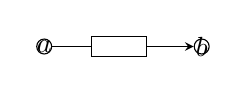
\begin{tikzpicture}

\ionode{(io1)}{(0,0)}{node {$a$}} 
\ionode{(io2)}{(2,0)}{node {$b$}}

\fifoe{(io1)}{(io2)}{}

\end{tikzpicture}
\end{center}
\vspace{0.5cm}
\end{minipage}
\begin{minipage}[b]{0.58\linewidth}
\begin{verbatim}
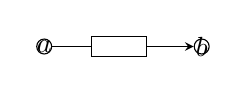
\begin{tikzpicture}
   \ionode{(io1)}{(0,0)}{node {$a$}} 
   \ionode{(io2)}{(2,0)}{node {$b$}}
   \fifoe{(io1)}{(io2)}{}
\end{tikzpicture}
\end{verbatim}
\end{minipage}

\bigskip

Ups! That is not what we desired!

In fact, the code \verb+node {<text>}+ creates a label right in the centre of the node to which it will be stick. 
This would result in almost invisible labels. 
The solution is to use position options. 
Such position options are thoroughly documented in the tikz \& pgf manual. Those presented next are easily understandable, and are enough to place the labels in desired positions:

\begin{itemize}
\item yshift or xshift: these options require a dimension $d$ and they make the label to move $d$ units in the vertical or horizontal axes, respectively. They should be used as: \verb+yshift=10pt+, for instance (the same notation is used for for the xshift, as it would be expected.

\item above, below, left right: these options do not require any value as they actually place the label in the expected positions. It may be, however,  needed that these options are used with the y or xshift to place the label in a more suitable position.

\end{itemize}

Take a look at the next example to understand how these options are used.


\bigskip

\begin{minipage}[b]{0.3\linewidth}
\begin{center}
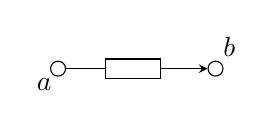
\begin{tikzpicture}

\ionode{(io1)}{(0,0)}{node[below, xshift=-5pt] {$a$}} 
\ionode{(io2)}{(2,0)}{node[yshift=8pt, xshift=5pt] {$b$}}

\fifoe{(io1)}{(io2)}{}

\end{tikzpicture}
\end{center}
\vspace{0.5cm}
\end{minipage}
\begin{minipage}[b]{0.68\linewidth}
\begin{verbatim}
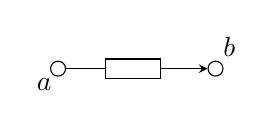
\begin{tikzpicture}
   \ionode{(io1)}{(0,0)}
     {node[below, xshift=-5pt] {$a$}} 
   \ionode{(io2)}{(2,0)}
     {node[yshift=8pt, xshift=5pt] {$b$}}
   \fifoe{(io1)}{(io2)}{}
\end{tikzpicture}
\end{verbatim}
\end{minipage}

\bigskip


It may be interesting to have some (read: more than one) labels in a node or in a channel. The next example shows how more than one label may be added to a channel, defining the stochastic LossySync channel with the stochastic annotations.
\paragraph{Note.} Since nodes and channels use the same notation to define labels, the code (the label parts) shown here may be applied to nodes too.


\bigskip

\begin{minipage}[b]{0.3\linewidth}
\begin{center}
\begin{tikzpicture}

\lossysync{(0,0)}{(2,0)}
			{node[above]{\tiny$\gamma ab$} 
			 node[below]{\tiny$\gamma aL$}
			 node[above, xshift=-30pt]{\tiny$\gamma a$}
			 node[above, xshift=30pt]{\tiny$\gamma b$}
			}

\end{tikzpicture}
\end{center}
\vspace{1.3cm}
\end{minipage}
\begin{minipage}[b]{0.68\linewidth}
\begin{verbatim}
\begin{tikzpicture}
   \lossysync{(0,0)}
             {(2,0)}
             {node[above]
           	 {\tiny$\gamma ab$} 
             node[below]
             {\tiny$\gamma aL$}
             node[above, xshift=-30pt]
             {\tiny$\gamma a$}
             node[above, xshift=30pt]
             {\tiny$\gamma b$}
     }
\end{tikzpicture}
\end{verbatim}
\end{minipage}


\bigskip

By the way it is possible to change the colour of the label, by adding to the node options the name of a colour. See how in the next example.


\bigskip

\begin{minipage}[b]{0.3\linewidth}
\begin{center}
\begin{tikzpicture}

\lossysync{(0,0)}{(2,0)}
          {node[above]{\tiny$\gamma ab$} 
           node[below, red]{\tiny$\gamma aL$}
          }

\end{tikzpicture}
\end{center}
\vspace{0.4cm}
\end{minipage}
\begin{minipage}[b]{0.68\linewidth}
\begin{verbatim}
\begin{tikzpicture}
  \lossysync{(0,0)}{(2,0)}
      {node[above]{\tiny$\gamma ab$} 
       node[below, red]{\tiny$\gamma aL$}
      }
\end{tikzpicture}
\end{verbatim}
\end{minipage}


\bigskip




\section{Summary}

In this document you learned how to use the reotex package, which allows for the construction of Reo Circuits, using Reo Channels and Nodes.

All the channels follow the same Channel API: receive a start point or a reference to such a start point (always between parentheses), then they receive a list of space-separated labels, and finally they receive the target point or the reference to that point.

The channels have a starred version that defines the existence, or not, of an arrow tip. 

The nodes (there are three different) also follow the same Node API: receive  a reference name (always between parentheses, composed of one or more words), then they receive the point and finally the list of space-separated labels.


Moreover, there are some special utility commands that allow for the construction of U- and L-shaped Channels. 



\bibliographystyle{plain}
\bibliography{../../../Reports/Reo/reo}


\end{document}









